\documentclass[12pt,fleqn]{article}\usepackage{../../common}
\begin{document}
Zaman Serisi Veri Analizi

Daha fazla ilerlemeden bu yazıda bazı veri işlem numaraları göreceğiz.

Durağanlığı Çıkartmak

Yapay Öğrenim (machine learning) ya da diğer istatistiki tahminsel yaklaşımlar
çoğunlukla işledikleri verinin durağan olmasının beklerler [1]. Durağanlık
zaman serisindeki her veri noktasının diğerleri ile aynı dağılıma sahip olması
demektir. Bunun tersini farzeden algoritmalar için bu rahatsızlık yaratır. 

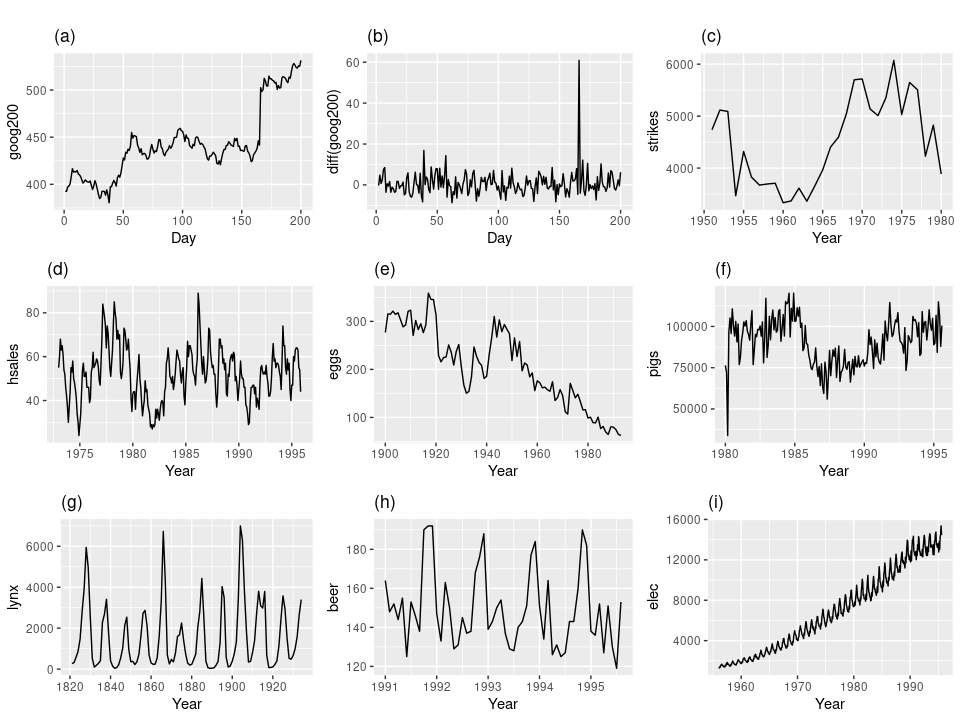
\includegraphics[width=25em]{tser_008_data_01.png}












[devam edecek]

Kaynaklar

[1] {\em How to Remove Non-Stationarity From Time Series},
    \url{https://www.kaggle.com/code/bextuychiev/how-to-remove-non-stationarity-from-time-series?scriptVersionId=73876070}

\end{document}
